% !TeX root = ../main.tex
% Add the above to each chapter to make compiling the PDF easier in some editors.

\chapter{Background}\label{chapter:background} % Anshul 4 sayfa yazmış

\section{Cloud Computing Landscape} % Cloud usage scenarios
\subsection{Usage Scenarios}
Cloud computing is becoming increasingly popular as on-demand provisioning capabilities and support for various use cases are growing. Cloud computing is currently being used in many different aspects of our lives. \cite{cloud-use-cases} Some of those aspects include file storage like OneDrive, database as a service systems like Amazon SimpleDB, entertainment services such as Netflix, multiplayer online games like Dota 2. Businesses are also using cloud computing for instant messaging between departments through applications like Slack or storing customer data in customer relationship management services provided by companies such as SAP or Salesforce. Many businesses also offload their computing requirements to cloud for data mining or for project management, as the Pay-per-use model of cloud is very beneficial for companies because they don't need to maintain a cluster of computers in premise. Cloud computing is also being used to host massive websites such as Facebook.com or Amazon.com.
\subsection{Virtualization}
The different use cases explained above are only possible because cloud computing provides abstraction by virtualisation. Real hardware in data centers can be abstracted and be broken to smaller units and be distributed to customers as virtual machines. That way every customer can have their own personal computer running on the cloud and their system is fully isolated from other customers. While virtual machines were the defacto unit in cloud computing for many years, now there is a new technology called \textit{containerisation}. Contaniers allow applications to be packed with their dependencies, and those application can run on the same host OS on top of a container engine. That allows for better utilized servers and less dependency from the underlying hardware. It comes with a cost though. Containers add another layer of abstraction on the stack thus they have a delay. 

This abstraction is possible with hypervisor technologies such as Xen. Controlled by software APIs, hypervisors boot self-contained computers on demand, and can run applications as if they were running on physical hosts. This is called \textit{server consolidation} and it has been a great way to reduce under-utilized hardware.

\section{Unikernels}
Unikernels \cite{library-operating-system} are specialised machine images compiled from high-level languages. Those machine images can run directly on the hypervisor or on the bare metal. 
\begin{figure}[htpb]
  \
  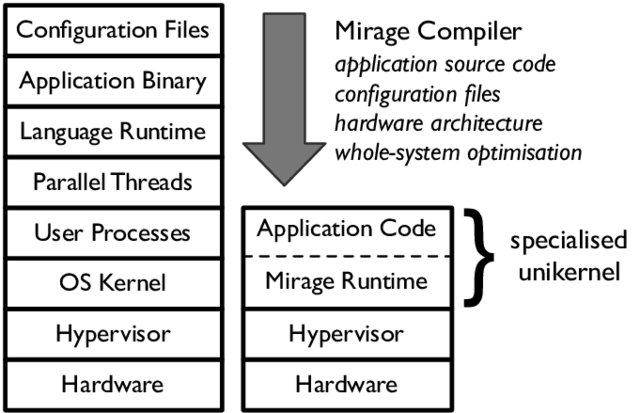
\includegraphics[height=0.3\textwidth]{figures/Contrasting-software-layers-in-existing-VM-appliances-vs-unikernels-standalone-kernel_W640.jpg} 
  \caption{ Contrasting software layers in existing VM appliances vs. unikernel’s standalone kernel compilation approach. \cite{library-operating-system}} \label{fig:unikernel-arch}
\end{figure}
% Todo: write more

\begin{figure}[htpb]
    \centering
    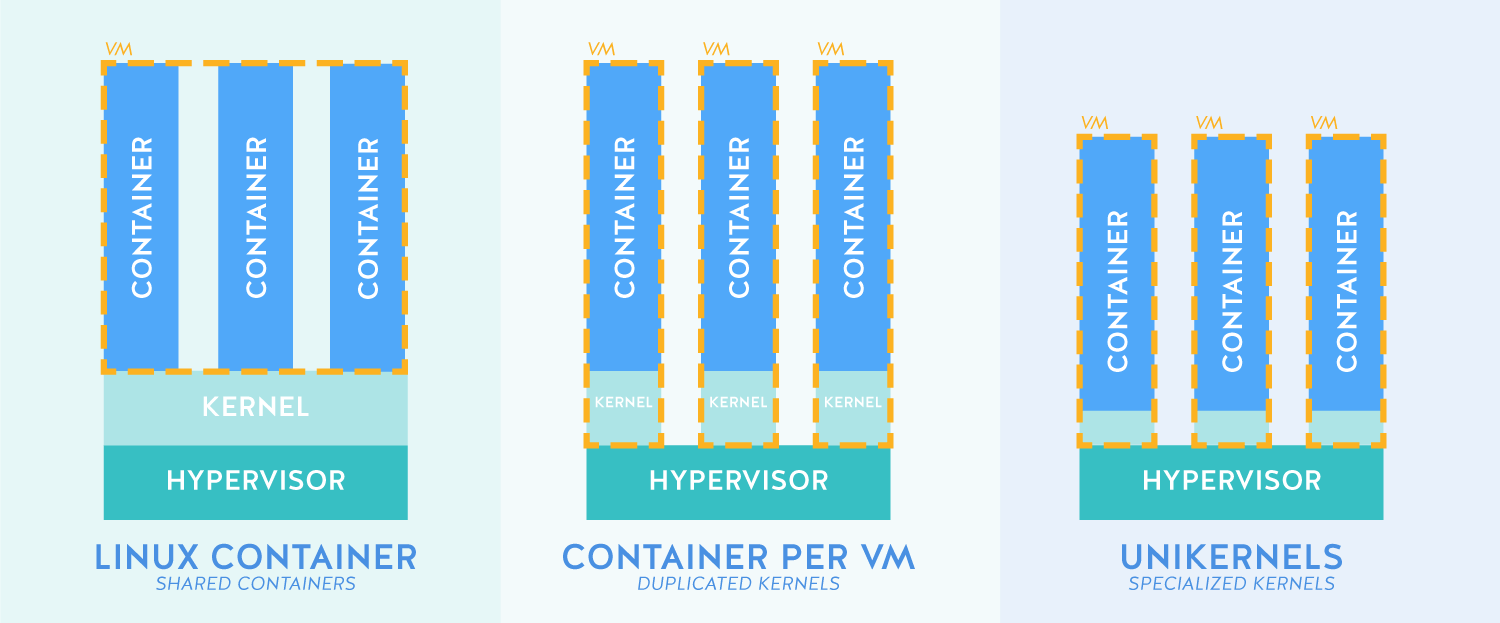
\includegraphics[width=0.4\textwidth]{figures/Linux-containers-vms-unikernels.png}
    \caption{Different virtualization techniques: https://nordicapis.com/introduction-to-unikernels/} \label{fig:virt}
  \end{figure}

\section{Orchestration}

\section{Managing IoT}
